\documentclass{article}
\usepackage{titling}
\usepackage{lipsum}
\usepackage{amsmath}
\usepackage{listings}
\usepackage{graphicx}
\usepackage{subcaption}
\usepackage{pgfplots}
\usepackage[margin=1in]{geometry}
\usepgfplotslibrary{statistics}



\begin{document}
\noindent
\begin{minipage}[t]{0.6\textwidth}
    \begin{flushleft}
        \LARGE\textbf{Math 343 - Lab 4} \\
        \vspace{6pt} % add 6pt of vertical space
        \hrule width 10cm
        \vspace{12pt}
        \large\textbf{Preston Duffield} \\
        \large Western Washington University \\
        \today
        % April 18, 2023
        \vspace{24pt}
    \end{flushleft}
\end{minipage}

\section*{Question 1}
\subsection*{a)}
To compute $\hat{\tau}_2$, note that:
\begin{align*}
    \hat{\tau}_2 &= \bar{y}_{2 \cdot} - \bar{y}_{\cdot \cdot} \\
                 &= 68.5 - 71.75 \\
                 &= -3.25 \\
\end{align*}
To compute $\hat{y}_{2 3}$, note that:
\begin{align*}
    \hat{y}_{2 3} &= \bar{y}_{2 \cdot} + \bar{y}_{\cdot 3} - \bar{y}_{\cdot \cdot} \\
                 &= 68.5 + 72.4 - 71.75 \\
                 &= 69.15 \\
\end{align*}
\subsection*{b)}
$H_0$: $\tau_1 = \tau_2 = \tau_3 = \tau_4 = 0$.\\
$H_a$: Not all $\tau_i = 0$.\\
An F test on the equality in mean effect (tensile strength of cloth after treatment) of the four
chemical agents gives an F-value = 2.38, and a p-value of 0.121, from which we can conclude the following.
There is not enough statistical evidence to support the hypothesis that not all $\tau_i = 0$.
\subsection*{c)}
$H_0$: The data are drawn from a normal distribution. \\
$H_a$: The data are not drawn from a normal distribution.\\
The residual plot does not appear to be linear. It seems to have an "S" shaped curve. The p-value $= 0.049 > \alpha = 0.01$, therefore, 
the evidence from the data is consistent with the hypothesis that the data are drawn from a normal distribution.
\subsection*{d)}
The graphical results of the Tukey pairwise comparison for every pair of the chemical treatments is:
\\
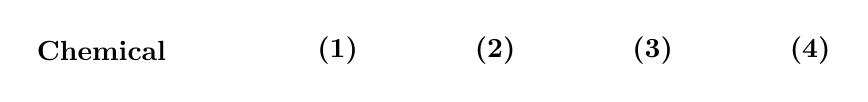
\begin{tikzpicture}[yscale=-1]
    % Define the positions of the labels
    \coordinate (labelPos) at (0, 0);
    \coordinate (1Pos) at (3, 0);
    \coordinate (2Pos) at (5, 0);
    \coordinate (3Pos) at (7, 0);
    \coordinate (4Pos) at (9, 0);

    % Draw the labels
    \node at (labelPos) {\textbf{Chemical}}; % Treatment label
    \node at (1Pos) {\textbf{(1)}};
    \node at (2Pos) {\textbf{(2)}};
    \node at (3Pos) {\textbf{(3)}};
    \node at (4Pos) {\textbf{(4)}};

    % Draw the line
    % \draw[ultra thick] ([yshift=0.5cm]3Pos) -- ([yshift=0.5cm]1Pos);
    % \draw[thick] ([yshift=1cm]1Pos) -- ([yshift=1cm]2Pos); % another theoretical line.
\end{tikzpicture}

Tukeys test threshold is:
\begin{align*}
    q_{\alpha, a, (a-1)(b-1)} \frac{s}{\sqrt{b}} &= q_{.05, 4, 12} \frac{\sqrt{1.817}}{\sqrt{5}}  \\
                                                 &= 4.20 (0.602)  \\
                                                 &= 2.531  \\
\end{align*}


\subsection*{e)}
Note that there is no line, this indicates that no means are significantly different. This is consistent with the above F-test which concluded that each treatment effect was equal to 0.


\section*{Question 2}
\subsection*{a)}
\subsection*{b)}
\subsection*{c)}
\subsection*{d)}


\end{document}